\documentclass[11pt,a4paper]{article}

\usepackage[utf8]{inputenc}
\usepackage[T1]{fontenc}
\usepackage{amsmath,amssymb,amsthm}
\usepackage{algorithm}
\usepackage{algpseudocode}
\usepackage{booktabs}
\usepackage{hyperref}
\usepackage[margin=2.5cm]{geometry}
\usepackage{natbib}
\usepackage{tikz}
\usetikzlibrary{arrows.meta,positioning,fit,backgrounds}

\newtheorem{theorem}{Theorem}
\newtheorem{proposition}{Proposition}
\newtheorem{definition}{Definition}
\newtheorem{remark}{Remark}

\title{Decomposition Methods in Maximum Satisfiability:\\
       Connecting Core-Guided and Implicit Hitting Set Algorithms\\
       with Benders and Dantzig--Wolfe Decomposition}

\author{Technical Report}

\date{May 2026}

\begin{document}

\maketitle

\begin{abstract}
Maximum Satisfiability (MaxSAT) and Mixed-Integer Programming (MIP) are two
major frameworks for combinatorial optimization that have largely developed in
separate communities. In this report we draw explicit structural parallels
between two families of MaxSAT algorithms and two classical decomposition
methods from operations research. We show that core-guided MaxSAT algorithms
operate as instances of Logic-Based Benders Decomposition (LBBD), where
unsatisfiable cores play the role of Benders cuts derived via inference duality.
Dually, we argue that Implicit Hitting Set (IHS) MaxSAT solvers implement a
form of Dantzig--Wolfe decomposition when viewed through LP duality, with the
SAT oracle acting as a pricing subproblem that generates new constraints
(columns in the dual). These connections unify the algorithmic landscape across
the two communities and suggest avenues for cross-fertilization.
\end{abstract}

%----------------------------------------------------------------------
\section{Introduction}
\label{sec:intro}
%----------------------------------------------------------------------

Maximum Satisfiability (MaxSAT) is the optimization version of the Boolean
Satisfiability problem (SAT): given a set of hard clauses~$\mathcal{H}$ and a
set of weighted soft clauses~$(\mathcal{S}, w)$, find a truth assignment that
satisfies all hard clauses while maximizing the total weight of satisfied soft
clauses (equivalently, minimizing the cost of falsified soft clauses).

Modern exact MaxSAT solvers fall into two broad families:
\begin{enumerate}
\item \textbf{Core-guided algorithms} (e.g., WPM1~\citep{ansotegui2009solving}, PMRES~\citep{narodytska2014maximum}, OLL~\citep{morgado2014core}), which iteratively call a SAT solver, extract unsatisfiable cores, and transform the formula to raise a lower bound.
\item \textbf{Implicit Hitting Set (IHS) algorithms} (e.g., MaxHS~\citep{davies2011solving,davies2013exploiting}), which alternate between a SAT oracle that extracts cores and an IP solver that computes a minimum-cost hitting set of the cores found so far.
\end{enumerate}

In operations research, Benders decomposition~\citep{benders1962partitioning}
and Dantzig--Wolfe decomposition~\citep{dantzigwolfe1960} are two classical
methods for structured optimization problems. Both decompose a hard monolithic
problem into a coordinating master problem and simpler subproblems, iterating
by passing cuts or columns between them. They are linked through LP
duality: Benders adds \emph{rows} (cuts) to a master problem defined over
complicating variables, while Dantzig--Wolfe adds \emph{columns} to a master
problem defined over complicating constraints.

The purpose of this report is to make explicit the structural correspondences:
\begin{itemize}
\item Core-guided MaxSAT $\longleftrightarrow$ Logic-Based Benders Decomposition,
\item IHS MaxSAT $\longleftrightarrow$ Dantzig--Wolfe Decomposition (in the dual).
\end{itemize}

%----------------------------------------------------------------------
\section{Preliminaries}
\label{sec:prelim}
%----------------------------------------------------------------------

\subsection{MaxSAT}

\begin{definition}[Weighted Partial MaxSAT]
An instance is a triple $\langle \mathcal{H}, \mathcal{S}, w \rangle$ where
$\mathcal{H}$ is a set of hard clauses, $\mathcal{S} = \{s_1, \ldots, s_m\}$
is a set of soft clauses, and $w : \mathcal{S} \to \mathbb{Q}_{>0}$ assigns
weights. A solution is an assignment $\sigma$ satisfying all clauses in
$\mathcal{H}$; its cost is $\sum_{s_i \,:\, \sigma \not\models s_i} w(s_i)$.
The goal is to find a minimum-cost solution.
\end{definition}

\begin{definition}[Core]
A \emph{core} of $\langle \mathcal{H}, \mathcal{S}, w \rangle$ is a subset
$\kappa \subseteq \mathcal{S}$ such that $\mathcal{H} \cup \kappa$ is
unsatisfiable. A core is \emph{minimal} (a MUS) if no proper subset is also a
core.
\end{definition}

\begin{definition}[Correction Set]
A \emph{correction set} is a subset $\mathcal{C} \subseteq \mathcal{S}$ whose
removal makes the formula satisfiable, i.e., $\mathcal{H} \cup (\mathcal{S}
\setminus \mathcal{C})$ is satisfiable. A correction set is \emph{minimal}
(an MCS) if no proper subset has this property.
\end{definition}

There is a well-known duality: every minimal core hits every minimal correction set, and vice versa~\citep{liffiton2008algorithms}.

\subsection{The LP Relaxation of MaxSAT}

Introduce a binary variable $y_i \in \{0,1\}$ for each soft clause $s_i$,
where $y_i = 1$ means $s_i$ is falsified. The MaxSAT problem can be written as
the integer program:
\begin{align}
\min \quad & \sum_{i=1}^{m} w(s_i)\, y_i \label{eq:maxsat-obj}\\
\text{s.t.} \quad & \sum_{s_i \in \kappa} y_i \geq 1 \quad \forall \text{ cores } \kappa, \label{eq:maxsat-core}\\
& y_i \in \{0,1\}. \label{eq:maxsat-int}
\end{align}
Constraint~\eqref{eq:maxsat-core} states that every core must be ``hit'' by
at least one falsified soft clause. This is the \emph{hitting set}
formulation, and there are exponentially many core constraints. The LP
relaxation replaces~\eqref{eq:maxsat-int} with $0 \leq y_i \leq 1$.

\subsection{Benders Decomposition}

Classical Benders decomposition~\citep{benders1962partitioning} partitions
variables into complicating variables~$x$ and easy variables~$y$. The master
problem optimizes over~$x$; for each fixed~$\bar{x}$, a subproblem over~$y$
either certifies feasibility or returns a \emph{Benders cut} derived from the
subproblem's dual. Cuts are accumulated in the master.

\emph{Logic-Based Benders Decomposition} (LBBD)~\citep{hooker2003logic}
generalizes this by allowing the subproblem to be any optimization or
feasibility problem. Cuts are derived via an \emph{inference dual}: any proof
of infeasibility or suboptimality of the subproblem yields a valid cut for the
master. The cut need not come from LP duality; it can come from any sound
deduction system.

\subsection{Dantzig--Wolfe Decomposition}

Dantzig--Wolfe decomposition~\citep{dantzigwolfe1960} addresses problems with
complicating \emph{constraints}. The feasible region of a subproblem is
represented via its extreme points. A restricted master problem uses a subset
of these extreme points (columns); a \emph{pricing subproblem} identifies
whether any extreme point with negative reduced cost exists. If so, the
corresponding column is added to the master. The procedure terminates when no
such column exists.

Through LP duality, Benders and Dantzig--Wolfe are intimately related: adding a
row (cut) to the primal master is equivalent to adding a column to the dual
master, and vice versa.

%----------------------------------------------------------------------
\section{Core-Guided MaxSAT as Benders Decomposition}
\label{sec:benders}
%----------------------------------------------------------------------

\subsection{The Decomposition Structure}

A core-guided MaxSAT algorithm operates in the following loop:
\begin{enumerate}
\item \textbf{Subproblem (SAT oracle):} Given the current (transformed) formula, call a SAT solver. If satisfiable, the model is optimal; stop. If unsatisfiable, obtain a core~$\kappa$.
\item \textbf{Master update:} Use the core~$\kappa$ to transform the formula (add relaxation variables, cardinality constraints) so that the lower bound increases.
\item Repeat.
\end{enumerate}

We now map this onto the LBBD framework of \citet{hooker2003logic}.

\begin{center}
\begin{tabular}{lll}
\toprule
\textbf{LBBD component} & \textbf{Core-guided MaxSAT analog} \\
\midrule
Complicating variables $x$ & Soft clause falsification decisions $y_i$ \\
Master problem & Accumulated lower bound + constraints \\
Subproblem $\mathrm{SP}(\bar{x})$ & SAT call on $\mathcal{H} \cup \mathcal{S}'$ \\
Infeasibility certificate & Unsatisfiable core $\kappa$ \\
Benders cut & Hitting set constraint: $\sum_{s_i \in \kappa} y_i \geq 1$ \\
Inference dual & SAT proof of unsatisfiability (e.g., resolution) \\
\bottomrule
\end{tabular}
\end{center}

\subsection{The Inference Dual Perspective}

In classical Benders, the cut $\pi^T b \leq z$ is derived from the LP dual of
the subproblem. In LBBD, the cut comes from any valid proof. In core-guided
MaxSAT, the SAT solver provides a refutation proof (via conflict-driven clause
learning) that establishes the unsatisfiability of $\mathcal{H} \cup \kappa$.
This proof serves as the solution to the inference dual: it certifies that
\emph{at least one} soft clause in $\kappa$ must be falsified, producing the
cut
\[
\sum_{s_i \in \kappa} y_i \geq 1.
\]
This is a \emph{combinatorial Benders cut}~\citep{hooker2003logic,codato2006combinatorial}: a linear inequality derived from a logical deduction rather than from LP duality.

\subsection{Formula Transformation as Implicit Cut Accumulation}

Core-guided solvers such as PMRES and OLL do not maintain an explicit master
IP. Instead, they transform the formula by adding relaxation variables and
cardinality constraints. Recent work by \citet{katsirelos2023analysis} has
shown that these transformations implicitly encode an LP. Specifically:

\begin{proposition}[\citeauthor{katsirelos2023analysis}, 2023]
The transformations performed by PMRES and OLL implicitly discover cores of the
original formula. In unweighted instances, the relaxed formula at each
iteration encodes a minimum hitting set of these cores. Moreover, the process
can be captured by a compact integer linear program whose LP relaxation yields
the same bound.
\end{proposition}

Thus, what appears to be a purely syntactic formula transformation is, in
fact, an implicit construction of the Benders master problem, with each core
extraction step corresponding to one iteration of the LBBD loop.

\begin{figure}[t]
\centering
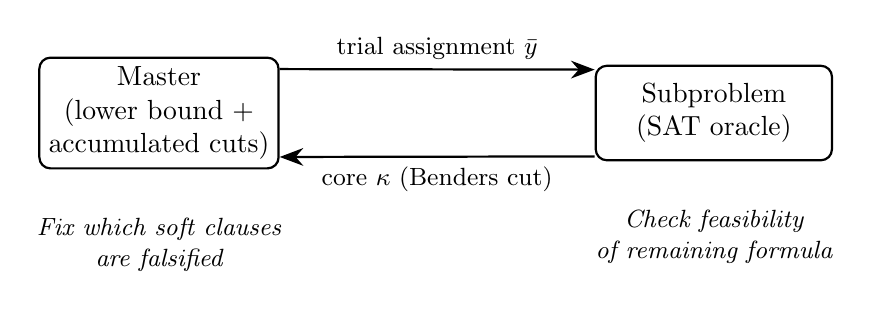
\begin{tikzpicture}[
    node distance=2.5cm and 4cm,
    block/.style={draw, rounded corners, minimum width=3cm, minimum height=1.2cm, align=center, thick},
    arrow/.style={-{Stealth[length=3mm]}, thick},
]
    \node[block] (master) {Master\\(lower bound +\\accumulated cuts)};
    \node[block, right=of master] (sub) {Subproblem\\(SAT oracle)};

    \draw[arrow] (master.20) -- node[above,font=\small] {trial assignment $\bar{y}$} (sub.160);
    \draw[arrow] (sub.200) -- node[below,font=\small] {core $\kappa$ (Benders cut)} (master.340);

    \node[below=0.5cm of master,font=\small\itshape,align=center] {Fix which soft clauses\\are falsified};
    \node[below=0.5cm of sub,font=\small\itshape,align=center] {Check feasibility\\of remaining formula};
\end{tikzpicture}
\caption{Core-guided MaxSAT as Logic-Based Benders Decomposition. The SAT oracle acts as the subproblem; each unsatisfiable core yields a combinatorial Benders cut.}
\label{fig:benders}
\end{figure}

%----------------------------------------------------------------------
\section{IHS MaxSAT as Dantzig--Wolfe Decomposition}
\label{sec:dw}
%----------------------------------------------------------------------

\subsection{The Implicit Hitting Set Framework}

The IHS algorithm~\citep{davies2011solving,moreno2013implicit} operates as follows:
\begin{enumerate}
\item \textbf{Master problem (IP solver):} Compute a minimum-cost hitting set $H^*$ of all cores found so far. That is, solve
\[
\min \sum_{i=1}^{m} w(s_i)\, y_i \quad \text{s.t.} \quad \sum_{s_i \in \kappa_j} y_i \geq 1 \;\; \forall j = 1,\ldots,k, \quad y_i \in \{0,1\}.
\]
\item \textbf{Oracle (SAT solver):} Check whether removing the clauses in $H^*$ from $\mathcal{S}$ makes the formula satisfiable. If yes, $H^*$ is optimal; stop. If not, the SAT solver returns a new core $\kappa_{k+1}$ that is not hit by $H^*$.
\item Add $\kappa_{k+1}$ as a new constraint and repeat.
\end{enumerate}

\subsection{The Dantzig--Wolfe Connection via LP Duality}

To see the Dantzig--Wolfe structure, consider the LP dual of the hitting set
formulation~\eqref{eq:maxsat-obj}--\eqref{eq:maxsat-core}. Let $\mathcal{K} =
\{\kappa_1, \ldots, \kappa_N\}$ be the set of all cores, and let $\lambda_j
\geq 0$ be the dual variable for core $\kappa_j$. The dual LP is:
\begin{align}
\max \quad & \sum_{j=1}^{N} \lambda_j \label{eq:dual-obj}\\
\text{s.t.} \quad & \sum_{j \,:\, s_i \in \kappa_j} \lambda_j \leq w(s_i) \quad \forall i = 1,\ldots,m, \label{eq:dual-pack}\\
& \lambda_j \geq 0. \label{eq:dual-nn}
\end{align}
This is a \emph{packing} problem over cores: find a maximum-weight fractional
packing of cores subject to the capacity of each soft clause.

Since the number of cores~$N$ is exponential, this dual cannot be solved
directly. However, it has the structure required for \emph{column generation}
(the algorithmic engine of Dantzig--Wolfe decomposition):
\begin{itemize}
\item The \textbf{restricted master} is the dual LP~\eqref{eq:dual-obj}--\eqref{eq:dual-nn} restricted to the cores $\kappa_1, \ldots, \kappa_k$ discovered so far. Each core $\kappa_j$ corresponds to a \emph{column} (variable $\lambda_j$) in this dual.
\item The \textbf{pricing subproblem} asks: does there exist a core $\kappa$ not in the current restricted master that has positive reduced cost? In the dual~\eqref{eq:dual-obj}--\eqref{eq:dual-nn}, this amounts to finding a core $\kappa$ such that $\mathcal{H} \cup \kappa$ is unsatisfiable and $\kappa$ is not hit by the current primal solution. The SAT oracle answers exactly this question.
\end{itemize}

\begin{center}
\begin{tabular}{lll}
\toprule
\textbf{Dantzig--Wolfe component} & \textbf{IHS MaxSAT analog} \\
\midrule
Restricted master (dual) & Packing LP over known cores \\
Column & Core $\kappa_j$ (dual variable $\lambda_j$) \\
Pricing subproblem & SAT oracle: find unhit core \\
Negative reduced cost & Core not hit by current hitting set \\
\midrule
Restricted master (primal) & Hitting set IP over known cores \\
New constraint (row) & New core $\kappa_{k+1}$ \\
\bottomrule
\end{tabular}
\end{center}

\begin{proposition}
The IHS algorithm is a primal-side implementation of column generation on
the dual of the MaxSAT hitting set LP. Each new core discovered by the SAT
oracle acts simultaneously as:
\begin{enumerate}
\item a new \emph{row} (constraint) in the primal hitting set master, and
\item a new \emph{column} (variable) in the dual packing master.
\end{enumerate}
By LP duality, adding a row to the primal is equivalent to adding a column to
the dual. Hence the IHS algorithm is a Dantzig--Wolfe procedure on the dual
formulation.
\end{proposition}

\begin{figure}[t]
\centering
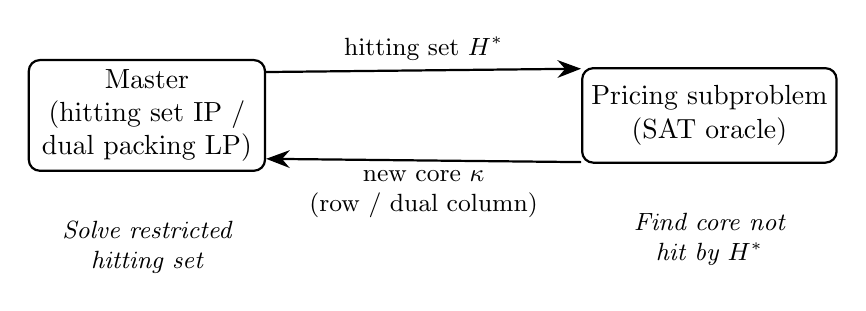
\begin{tikzpicture}[
    node distance=2.5cm and 4cm,
    block/.style={draw, rounded corners, minimum width=3cm, minimum height=1.2cm, align=center, thick},
    arrow/.style={-{Stealth[length=3mm]}, thick},
]
    \node[block] (master) {Master\\(hitting set IP /\\dual packing LP)};
    \node[block, right=of master] (sub) {Pricing subproblem\\(SAT oracle)};

    \draw[arrow] (master.20) -- node[above,font=\small] {hitting set $H^*$} (sub.160);
    \draw[arrow] (sub.200) -- node[below,font=\small,align=center] {new core $\kappa$\\(row / dual column)} (master.340);

    \node[below=0.5cm of master,font=\small\itshape,align=center] {Solve restricted\\hitting set};
    \node[below=0.5cm of sub,font=\small\itshape,align=center] {Find core not\\hit by $H^*$};
\end{tikzpicture}
\caption{IHS MaxSAT as Dantzig--Wolfe Decomposition (dual view). The SAT oracle acts as the pricing subproblem; each new core is a column in the dual packing LP.}
\label{fig:dw}
\end{figure}

\subsection{LP Bounds and Convergence}

In Dantzig--Wolfe decomposition, the restricted master LP provides a bound
that improves monotonically as columns are added, converging to the LP
optimum. Similarly, in IHS, adding more cores tightens the LP relaxation of
the hitting set master. \citet{davies2013exploiting} showed that solving the
hitting set master as an IP (rather than an LP) accelerates convergence
in practice by providing both primal feasible solutions and dual bounds
simultaneously.

The work of \citet{katsirelos2023analysis} further showed that core-guided
algorithms such as OLL implicitly compute feasible dual solutions of an LP
that encodes the same hitting set structure. This means that both families
of algorithms---core-guided and IHS---are optimizing over the \emph{same}
LP relaxation, but from opposite sides of duality.

%----------------------------------------------------------------------
\section{The Unified Picture}
\label{sec:unified}
%----------------------------------------------------------------------

The preceding analysis reveals a clean duality diagram connecting the four
methods:

\begin{figure}[h]
\centering
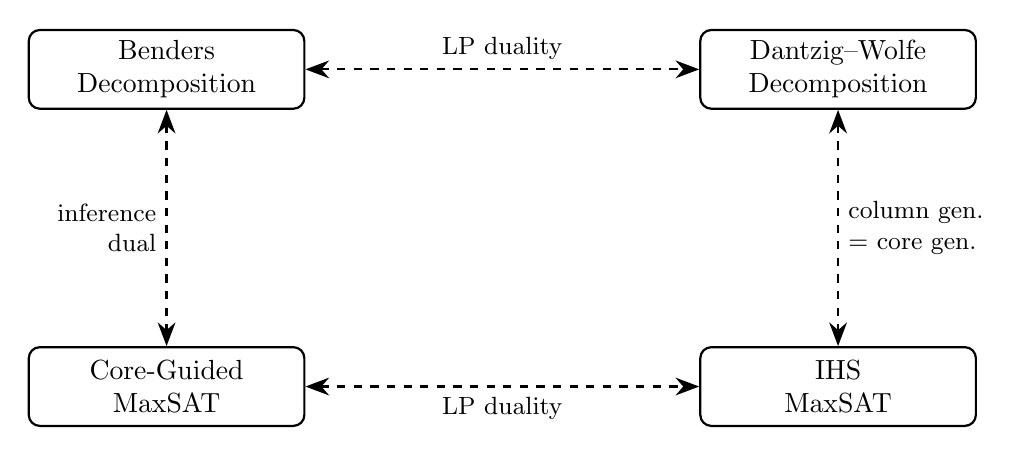
\begin{tikzpicture}[
    node distance=3cm and 5cm,
    block/.style={draw, rounded corners, minimum width=3.5cm, minimum height=1cm, align=center, thick},
    arrow/.style={{Stealth[length=3mm]}-{Stealth[length=3mm]}, thick, dashed},
]
    \node[block] (benders) {Benders\\Decomposition};
    \node[block, right=of benders] (dw) {Dantzig--Wolfe\\Decomposition};
    \node[block, below=of benders] (cg) {Core-Guided\\MaxSAT};
    \node[block, below=of dw] (ihs) {IHS\\MaxSAT};

    \draw[arrow] (benders) -- node[above,font=\small] {LP duality} (dw);
    \draw[arrow] (cg) -- node[below,font=\small] {LP duality} (ihs);
    \draw[arrow] (benders) -- node[left,font=\small,align=right] {inference\\dual} (cg);
    \draw[arrow] (dw) -- node[right,font=\small,align=left] {column gen.\\= core gen.} (ihs);
\end{tikzpicture}
\caption{The duality square connecting decomposition methods and MaxSAT algorithms.}
\label{fig:square}
\end{figure}

\begin{itemize}
\item \textbf{Horizontal axis (LP duality):} Benders and Dantzig--Wolfe are
dual to each other; core-guided and IHS are dual to each other in the same
sense. Adding a cut in one is adding a column in the other.
\item \textbf{Vertical axis (generalization):} Core-guided MaxSAT is an
instance of LBBD where the inference dual replaces the LP dual. IHS MaxSAT
is an instance of Dantzig--Wolfe where the pricing oracle is a SAT solver
rather than an LP.
\end{itemize}

This diagram also explains empirically observed complementarities. IHS solvers
(like Dantzig--Wolfe) tend to produce good primal solutions quickly because
the master IP yields feasible hitting sets at each iteration. Core-guided
solvers (like Benders) tend to produce strong dual bounds because each core
directly tightens the relaxation. This mirrors the well-known tradeoff in
OR between cut-based and column-based approaches.

%----------------------------------------------------------------------
\section{Discussion}
\label{sec:discussion}
%----------------------------------------------------------------------

\paragraph{Implications for algorithm design.}
The decomposition viewpoint suggests several ideas for improving MaxSAT
solvers:
\begin{enumerate}
\item \emph{Warm-starting}: In OR, Benders and Dantzig--Wolfe solvers
routinely warm-start the master with cuts or columns from heuristic solutions.
The same idea applies to MaxSAT: seeding the IHS master with cores from a
quick core-guided run, or vice versa.
\item \emph{Cut strengthening}: The Benders literature contains extensive work
on strengthening cuts (Pareto-optimal cuts, Magnanti--Wong cuts). Analogous
techniques could be applied to core minimization and core-guided clause
transformations.
\item \emph{Stabilization}: Column generation is notoriously unstable (the
``tailing-off'' effect). Stabilization techniques (dual penalties, bundle
methods) could improve IHS convergence.
\item \emph{Hybrid methods}: The recent SAT 2025 work of
\citet{katsirelos2025core} shows that OLL can be restated as an algorithm
that explicitly computes dual solutions of an LP, opening the door to hybrid
algorithms that interleave core-guided (Benders-like) and IHS
(Dantzig--Wolfe-like) steps within the same solve.
\end{enumerate}

\paragraph{Limitations.}
The analogy is structural, not exact. Core-guided solvers work with integer
formulas and perform syntactic transformations, not LP pivots. The IHS master
is typically solved as an IP, not an LP, which goes beyond standard column
generation. Moreover, the subproblem in both cases is a SAT call---an
NP-complete problem---rather than the polynomial-time LP solve assumed in
classical decomposition theory. Nonetheless, the structural parallels are
useful for transferring insights between communities.

%----------------------------------------------------------------------
\section{Conclusion}
\label{sec:conclusion}
%----------------------------------------------------------------------

We have presented explicit structural correspondences between two families of
MaxSAT algorithms and two classical decomposition methods from operations
research. Core-guided MaxSAT algorithms implement a form of Logic-Based
Benders Decomposition, where unsatisfiable cores serve as combinatorial
Benders cuts derived through inference duality. Implicit Hitting Set
algorithms implement a form of Dantzig--Wolfe decomposition (viewed through LP
duality), where the SAT oracle acts as a pricing subproblem generating new
columns in the dual packing formulation. These connections are mediated by LP
duality: the hitting set (primal) and core packing (dual) formulations of
MaxSAT stand in the same relationship as Benders and Dantzig--Wolfe masters.

Making these connections explicit opens a two-way transfer of techniques
between the OR and SAT communities, from cut strengthening and stabilization
to hybrid primal-dual algorithms that leverage the strengths of both
decomposition paradigms.

%----------------------------------------------------------------------
% References
%----------------------------------------------------------------------
\bibliographystyle{plainnat}

\begin{thebibliography}{20}

\bibitem[Ansotegui et~al.(2009)]{ansotegui2009solving}
C.~Ansotegui, M.L.~Bonet, and J.~Levy.
\newblock Solving (weighted) partial {MaxSAT} through satisfiability testing.
\newblock In \emph{Proc.\ SAT 2009}, LNCS 5584, pages 427--440. Springer, 2009.

\bibitem[Benders(1962)]{benders1962partitioning}
J.F.~Benders.
\newblock Partitioning procedures for solving mixed-variables programming
  problems.
\newblock \emph{Numerische Mathematik}, 4(1):238--252, 1962.

\bibitem[Codato and Fischetti(2006)]{codato2006combinatorial}
G.~Codato and M.~Fischetti.
\newblock Combinatorial {B}enders' cuts for mixed-integer linear programming.
\newblock \emph{Operations Research}, 54(4):756--766, 2006.

\bibitem[Dantzig and Wolfe(1960)]{dantzigwolfe1960}
G.B.~Dantzig and P.~Wolfe.
\newblock Decomposition principle for linear programs.
\newblock \emph{Operations Research}, 8(1):101--111, 1960.

\bibitem[Davies and Bacchus(2011)]{davies2011solving}
J.~Davies and F.~Bacchus.
\newblock Solving {MAXSAT} by solving a sequence of simpler {SAT} instances.
\newblock In \emph{Proc.\ CP 2011}, LNCS 6876, pages 225--239. Springer, 2011.

\bibitem[Davies and Bacchus(2013)]{davies2013exploiting}
J.~Davies and F.~Bacchus.
\newblock Exploiting the power of {MIP} solvers in {MaxSAT}.
\newblock In \emph{Proc.\ SAT 2013}, LNCS 7962, pages 166--181. Springer, 2013.

\bibitem[Hooker and Ottosson(2003)]{hooker2003logic}
J.N.~Hooker and G.~Ottosson.
\newblock Logic-based {B}enders decomposition.
\newblock \emph{Mathematical Programming}, 96(1):33--60, 2003.

\bibitem[Katsirelos(2023)]{katsirelos2023analysis}
G.~Katsirelos.
\newblock An analysis of core-guided maximum satisfiability solvers using linear
  programming.
\newblock In \emph{Proc.\ SAT 2023}, LIPIcs 271, pages 12:1--12:19. Dagstuhl, 2023.

\bibitem[Katsirelos(2025)]{katsirelos2025core}
G.~Katsirelos.
\newblock Core-guided linear programming-based maximum satisfiability.
\newblock In \emph{Proc.\ SAT 2025}, LIPIcs 341, pages 17:1--17:19. Dagstuhl, 2025.

\bibitem[Liffiton and Sakallah(2008)]{liffiton2008algorithms}
M.H.~Liffiton and K.A.~Sakallah.
\newblock Algorithms for computing minimal unsatisfiable subsets of constraints.
\newblock \emph{Journal of Automated Reasoning}, 40(1):1--33, 2008.

\bibitem[Moreno-Centeno and Karp(2013)]{moreno2013implicit}
E.~Moreno-Centeno and R.M.~Karp.
\newblock The implicit hitting set approach to solve combinatorial optimization
  problems with an application to multigenome alignment.
\newblock \emph{Operations Research}, 61(2):453--468, 2013.

\bibitem[Morgado et~al.(2014)]{morgado2014core}
A.~Morgado, C.~Dodaro, and J.~Marques-Silva.
\newblock Core-guided {MaxSAT} with soft cardinality constraints.
\newblock In \emph{Proc.\ CP 2014}, LNCS 8656, pages 564--573. Springer, 2014.

\bibitem[Morgado et~al.(2013)]{morgado2013iterative}
A.~Morgado, F.~Heras, M.~Liffiton, J.~Planes, and J.~Marques-Silva.
\newblock Iterative and core-guided {MaxSAT} solving: A survey and assessment.
\newblock \emph{Constraints}, 18(4):478--534, 2013.

\bibitem[Narodytska and Bacchus(2014)]{narodytska2014maximum}
N.~Narodytska and F.~Bacchus.
\newblock Maximum satisfiability using core-guided {MaxSAT} resolution.
\newblock In \emph{Proc.\ AAAI 2014}, pages 2717--2723. AAAI Press, 2014.

\bibitem[Narodytska et~al.(2022)]{narodytska2022cores}
N.~Narodytska, N.~Bj{\o}rner, M.-C.~Marinescu, and M.~Sagiv.
\newblock Analysis of core-guided {MaxSat} using cores and correction sets.
\newblock In \emph{Proc.\ SAT 2022}, LIPIcs 236, pages 26:1--26:20. Dagstuhl, 2022.

\end{thebibliography}

\end{document}
